% Chapter 2
\chapter[Experimental approach of surpressing the spectral diffusion]{Experimental approach of surpressing the spectral diffusion} % Main chapter title

\label{Chapter2} % Change X to a consecutive number; for referencing this chapter elsewhere, use \ref{ChapterX}

%----------------------------------------------------------------------------------------
%	SECTION 1
%----------------------------------------------------------------------------------------
\section{Information regarding the nanodiamond sample}

\paragraph{here is a paragraph about the fabrication of nanodiamond}
\FloatBarrier
\begin{figure}[h]
\centering
\includegraphics[width=0.7\linewidth]{Figures/pic/Unbenannt}
\caption{}
\label{fig:unbenannt}
\end{figure}
\FloatBarrier

\paragraph{here is a paragraph about the separation of the nanodiamonds}
\FloatBarrier
\begin{figure}[h]
\centering
\includegraphics[width=0.7\linewidth]{Figures/pic/Unbenannt1}
\caption{}
\label{fig:unbenannt1}
\end{figure}
\FloatBarrier
\section[sample preparation]{sample preparation}
\subsection{preparation of the substrate}
\paragraph{IIa diamond as substrate}

To choose a proper substrate for the nanodiamond sample, a few principles need to be considered.

\paragraph{1.}Low background fluorescence. 
It is always vital to obtain a decent signal to noise ration in any kind of meansurements. As for our case, the emission(fluorescence) from sillicon centers are the target, thus we would love to lower the back ground fluorescence as much as possilble.
\paragraph{2.}Good heat conductivity at low temperature.
From previous calculation done by Uwen Jantzen, we know that the temperature difference $\bigtriangleup T$ between the bottom of the substrate and nanodiamonds(which are spin coated on the surface of the substrate) can be estimate as\newline
$\bigtriangleup T = \frac{\sigma \cdot d \cdot T^{4}}{k} $,
where $\sigma$ is the Stefan–Boltzmann constant, $d$ is the thickness of the substrate and $k$ is the thermal conductivity.
To resolve the fine feature of sillicon vacancy ZPL, we want to characterise the nanodiamond sample at a temperature that is lower than 30K for spectrometer and 10K? for PLE.
\paragraph{3.} No distracting spectral features.
Some misleading peaks from the emission of the substrate would be the least wanted when we want to character a sample spectrally. In many cases, this is related to the raman-scattering of the photons, which highly depends on the crystal structure of the substrate. This scattering process alters the energy of the incident photons by shifts of concrete values and sometime can introduce peaks that are misleading or distracting.
\paragraph{4.}Refractive index. Inam et al calculated the relative emission rate for radiating dipoles near an interface between two dielectrics with FDTD simulation. The result demonstrates that in both of the cases, when the dipole lies prependicular and parallel to the substrate, the emission rate from a interface with lower relative refractive index is always higher than that from a interface with higher relative refractive index. And to increase the emission rate, a substrate with lower refractive index would be prefered.
\paragraph{}Prevously, taking these principles into consideration, my colleges have already ruled out a couple of materials, for instance, glass/quartz(distraction raman shift lines) and Sapphire(also a distracting raman shift line, and impurity induced emission that calls for extra attention when picking the optical filters). Now the temporary choice has landed on IIa type diamond, which has a low impurity density(resulting in low background fluorescence intensity), relatively low refractive index(2,4 to 2,7), good thermal conductivity($\bigtriangleup T = 4,17 \cdot 10^{-2}K$) and a raman shift at 1332$cm^{-1} $ that causes no distraction on our observation.

\paragraph{Focused Ion Beam milling}
In order to make it more convenient to trace the nanodiamonds, markers were curved onto the surface of the IIa type diamond substrate, this work was done by Uwe Jantzen during his master's thesis period. As is shown in the fig.[], the focues ion beam bombards the surface of diamond away and leaves behind markers that are visible in optical microscopy images and SEM images, as well as confocal microscopy images.
\paragraph{here is a sketch of how Ga-ion bombards the surface of substrate}
\paragraph{here insert image of markers, optical, sem and confocal}
\FloatBarrier
\begin{figure}[h]
\centering
\includegraphics[width=0.7\linewidth]{Figures/pic/20150907_sample214_spincoated_5}
\caption{}
\label{fig:20150907sample214spincoated5}
\end{figure}
\FloatBarrier
\begin{figure}[h]
\centering
\includegraphics[width=0.7\linewidth]{Figures/pic/20150917-132834_sample214_49_q00}
\caption{}
\label{fig:20150917-132834sample21449q00}
\end{figure}
\FloatBarrier
\begin{figure}[h]
\centering
\includegraphics[width=0.7\linewidth]{Figures/pic/2015-09-16_12h06m53s_confocal_xy_image_from_raw}
\caption{}
\label{fig:20150907sample214spincoated5}
\end{figure}
\FloatBarrier


\subsection{spin-coating of the sample}
\subsubsection{theory of spin coating} 
Spin coating is the method of sample preparing that mainly contains 2 steps:

1. Spreading of the liquid. In this step, certain volume of liquid containing the particle that we want to coat with is dropped on the surface of the substrate, driven by the centrifuging force from the rotational movement of the substrate, the liquid would be spread evenly on the surface.

2. Evaporation of the 'solvent'. While the sample stage rotates, the 'solvent'(In our case is not a real solvent, since nanodiamonds never really desolve.) would evaporate, leaving the particle/molecules that are wanted to be coated on the substrate.

In this procedure, 2 factors we find important.

1.spin speed: generally the thickness of the liquid layer $t$ is proportional to the inverse of the angular velocity $w$ squared t $\sim$ $\frac{1}{\sqrt{\omega}}$, higher speed would help with forming a more uniform layer, yet this also means a smaller volume of solution, which would lead to lower density of nanodiamonds of the surface. On the other hand, with lower speed, the probability of aggregation would increase, which is also what we want to prevent.

2.volume of the 'solution': larger volume means longer drying time, which would increase the probability of aggregation and losing nanodiamonds, while smaller volume leads towards lower density of nanodiamond and more difficulty when trying to drop it with a pipette. 

3.type of solvent: The type of solvent, viscosity and boiling point are important for the dispersion of nanoparticles inside solution, the spreading of the solution while spin coating and the rate of evaporation.

4.surface condition of the substrate. High contact angle is a obstacle towards the spreading of the solution, high roughness or inappropriate surface group of the substrate can result in poor wettability from the solution.

Throughout my project, with the help of Andrea Kurz, several combination of these factors had been has been tried out and in the end we landed on 

\paragraph{here we need a list of different program of spin coating that we have tried,with indexxxxx}

%-----------------------------------
\subsubsection{Acid cleaning}
To make sure that the NDs dispension can evenly spread and eventually settled on the substrate, a smooth, clean and hydrophilic surface is important.

Acid boiling is a very practicle way of diamond substrate cleaning. As it is called, the diamond will be boiled in a mixture of three strong mineral acids: sulfuric acid, nitric acid and perchloric acid. This mixture has ver strong ability of oxidizing.

\paragraph{here insert a sketch of how we do acid cleaning} 

After assembling the setup, we initialize the reaction by heating the mixture to a temperature where is mildly bubbles. The substrate would be stay inside the boiling tri-acid mix for 4h. 
The mixture of strong mineral oxidizing acid can remove most of the adhesions on the surface of diamond substrate , leaving a clean hydrphilic surface. This oxidizing procedure will lead to the formation of carbonyl and carboxyl groups.




\paragraph {here insert image of before and after cleaning substrate, optical image, confocal image }
\FloatBarrier
\begin{figure}[h]
\centering
\includegraphics[width=0.7\linewidth]{Figures/pic/image470}
\caption{}
\label{fig:image470}
\end{figure}
\FloatBarrier
fig. the comparision between before and after acid boiling(need to be inserted later).
 
Tri Acid boiling blabla. Expectation of the surface. Before after cleaning. Optical image. Confocal image.

%-----------------------------------
%	SECTION 2
%-----------------------------------
\section[development of a technology to estimate the spectral diffusion]{development of a technology to estimate the spectral diffusion}

\paragraph{Setup} 

In order to resolve the fine structure of ZPL of SiVs, we need to observe the sample at low temperature, thus a cryogenic setup must be applied.
Our setup is a typical confocal micropscopy setup connects with a cryostat, which cools the sample with liquid Helium flow.

\paragraph{here inserts a picture of our flow cryostat, from out and in side.}
This is the flow cryostat, whose main body is a vaccum chamber with

\paragraph{here insert a sketch of the cryo4 setup}
Confocal + Cryostat, Green laser + Red laser, spectrometer, apd, pic


\paragraph{PL} Photoluminescence spectra is one of the most efficient way of finding silicon vacancies. In this measurement, we use green laser of 532nm to excite the Silicon vacancies from ground state to 

\paragraph{PLE} resonance excitation of optical transition. Rsésolution limited by scanning step of laser. Observing phonon side band with apd. range of scanning: limited by laser, small.

\paragraph{time resolved PL spectra} Tracing PL spectra over time, show the diffusing behaviour of lines, characterisation methods: excitation polarisation: width of diffusion. Cross- correlation over time.
\paragraph{}We recorded and noticed that the diffusion, whose range can up to 1nm, is far beyond the capability of PLE. 

%-----------------------------------
%	SECTION 3
%-----------------------------------
\section{Oxidation}
\paragraph{Effect of Oxidation}
Room temperature oxidization is a common way of nanodiamond purification. With different oxidizing temperature, different types of impurities can be removed from the surface of the nanodiamond, ranging from water and physisorbed organic impurities, amourphous carbon, and graphitic shells and ultimate the $sp^{3}$ phase of diamond[T.Gaebel,2010]. After the oxidation, carbonyl and carboxyl groups are formed on the surface[Petrakov,2012]. Several paper have mentioned temperature choices for oxidation aiming at impurity removal. During the master's thesis period, 2 different oxidation has been examined.

\subsection[first Oxidation]{first Oxidation}
\paragraph{method}As reported, oxidation of $sp^{2}$ carbon already starts at $400^{o}C$, while the size reducing rate of diamond phase remains neglactable when the temperature is lower than $500^{o}C$. So it is an obvious choice to settle down the oxidation temperature at somewhere close to $500^{o}C$ when the maximum removal of $sp^{2}$ phased carbons and the minimum lost of the diamond body($sp^{3}$ phased carbons). Inspired by Elka Neu's paper, ....here insert a sentence explaining why we choose the two step oxidation program.
\paragraph{setup}

The aerobatic oxidation is carried out in a tube furnace that is offered by the ?? institute and it is done with the help of Markus Mohr. The tube furnace consists of a glass tube connected to the room atmosphere and heating coils around the glass tube. The glass tube is slidable. We put our sample inside a ceramic ?bowl? and put the bowl into the glass tube carefully, after the temperature has been raised to ?460C?, the glass tube would be slide into the heating coils. After the Oxidation, the glass tube would be slide out and the sample would cooled inside the tube until room temperature.

\paragraph{pre-characterisation}
Before the oxidation, we tried to characterise the sample with several different methods based on our confocal microscopy setup.

1. RT poi mapping

First we take a scan with green laser and record the fluorescence with an APD, which offers us a confocal microscopy image of the surface of the sample, then the photoluminescnce spectra of the bright spots are taken, those ones with a sharp peak at 737nm are saved as points of interests and their positions are saved as region of interest for the reference of further examine.
\FloatBarrier
\begin{figure}[h]
\centering
\includegraphics[width=0.7\linewidth]{Figures/pic/2015-09-07-ow-capture-20150907151210-744-1}
\caption{}
\label{fig:2015-09-07-ow-capture-20150907151210-744-1}
\end{figure}

\FloatBarrier

2. Cold spectra and PLE 
The sample is attached to an cold finger and the placed inside the cryostat, after UHV condition has been achieved, we start the helium transfer, which would brought the temperature of the sample down to 4.8K. We refound the points of interests that has been confirmed with SiV like spectra

3. PLE spectra

4.time-resolved PL spectra.
\FloatBarrier
\begin{figure}[h]
\centering
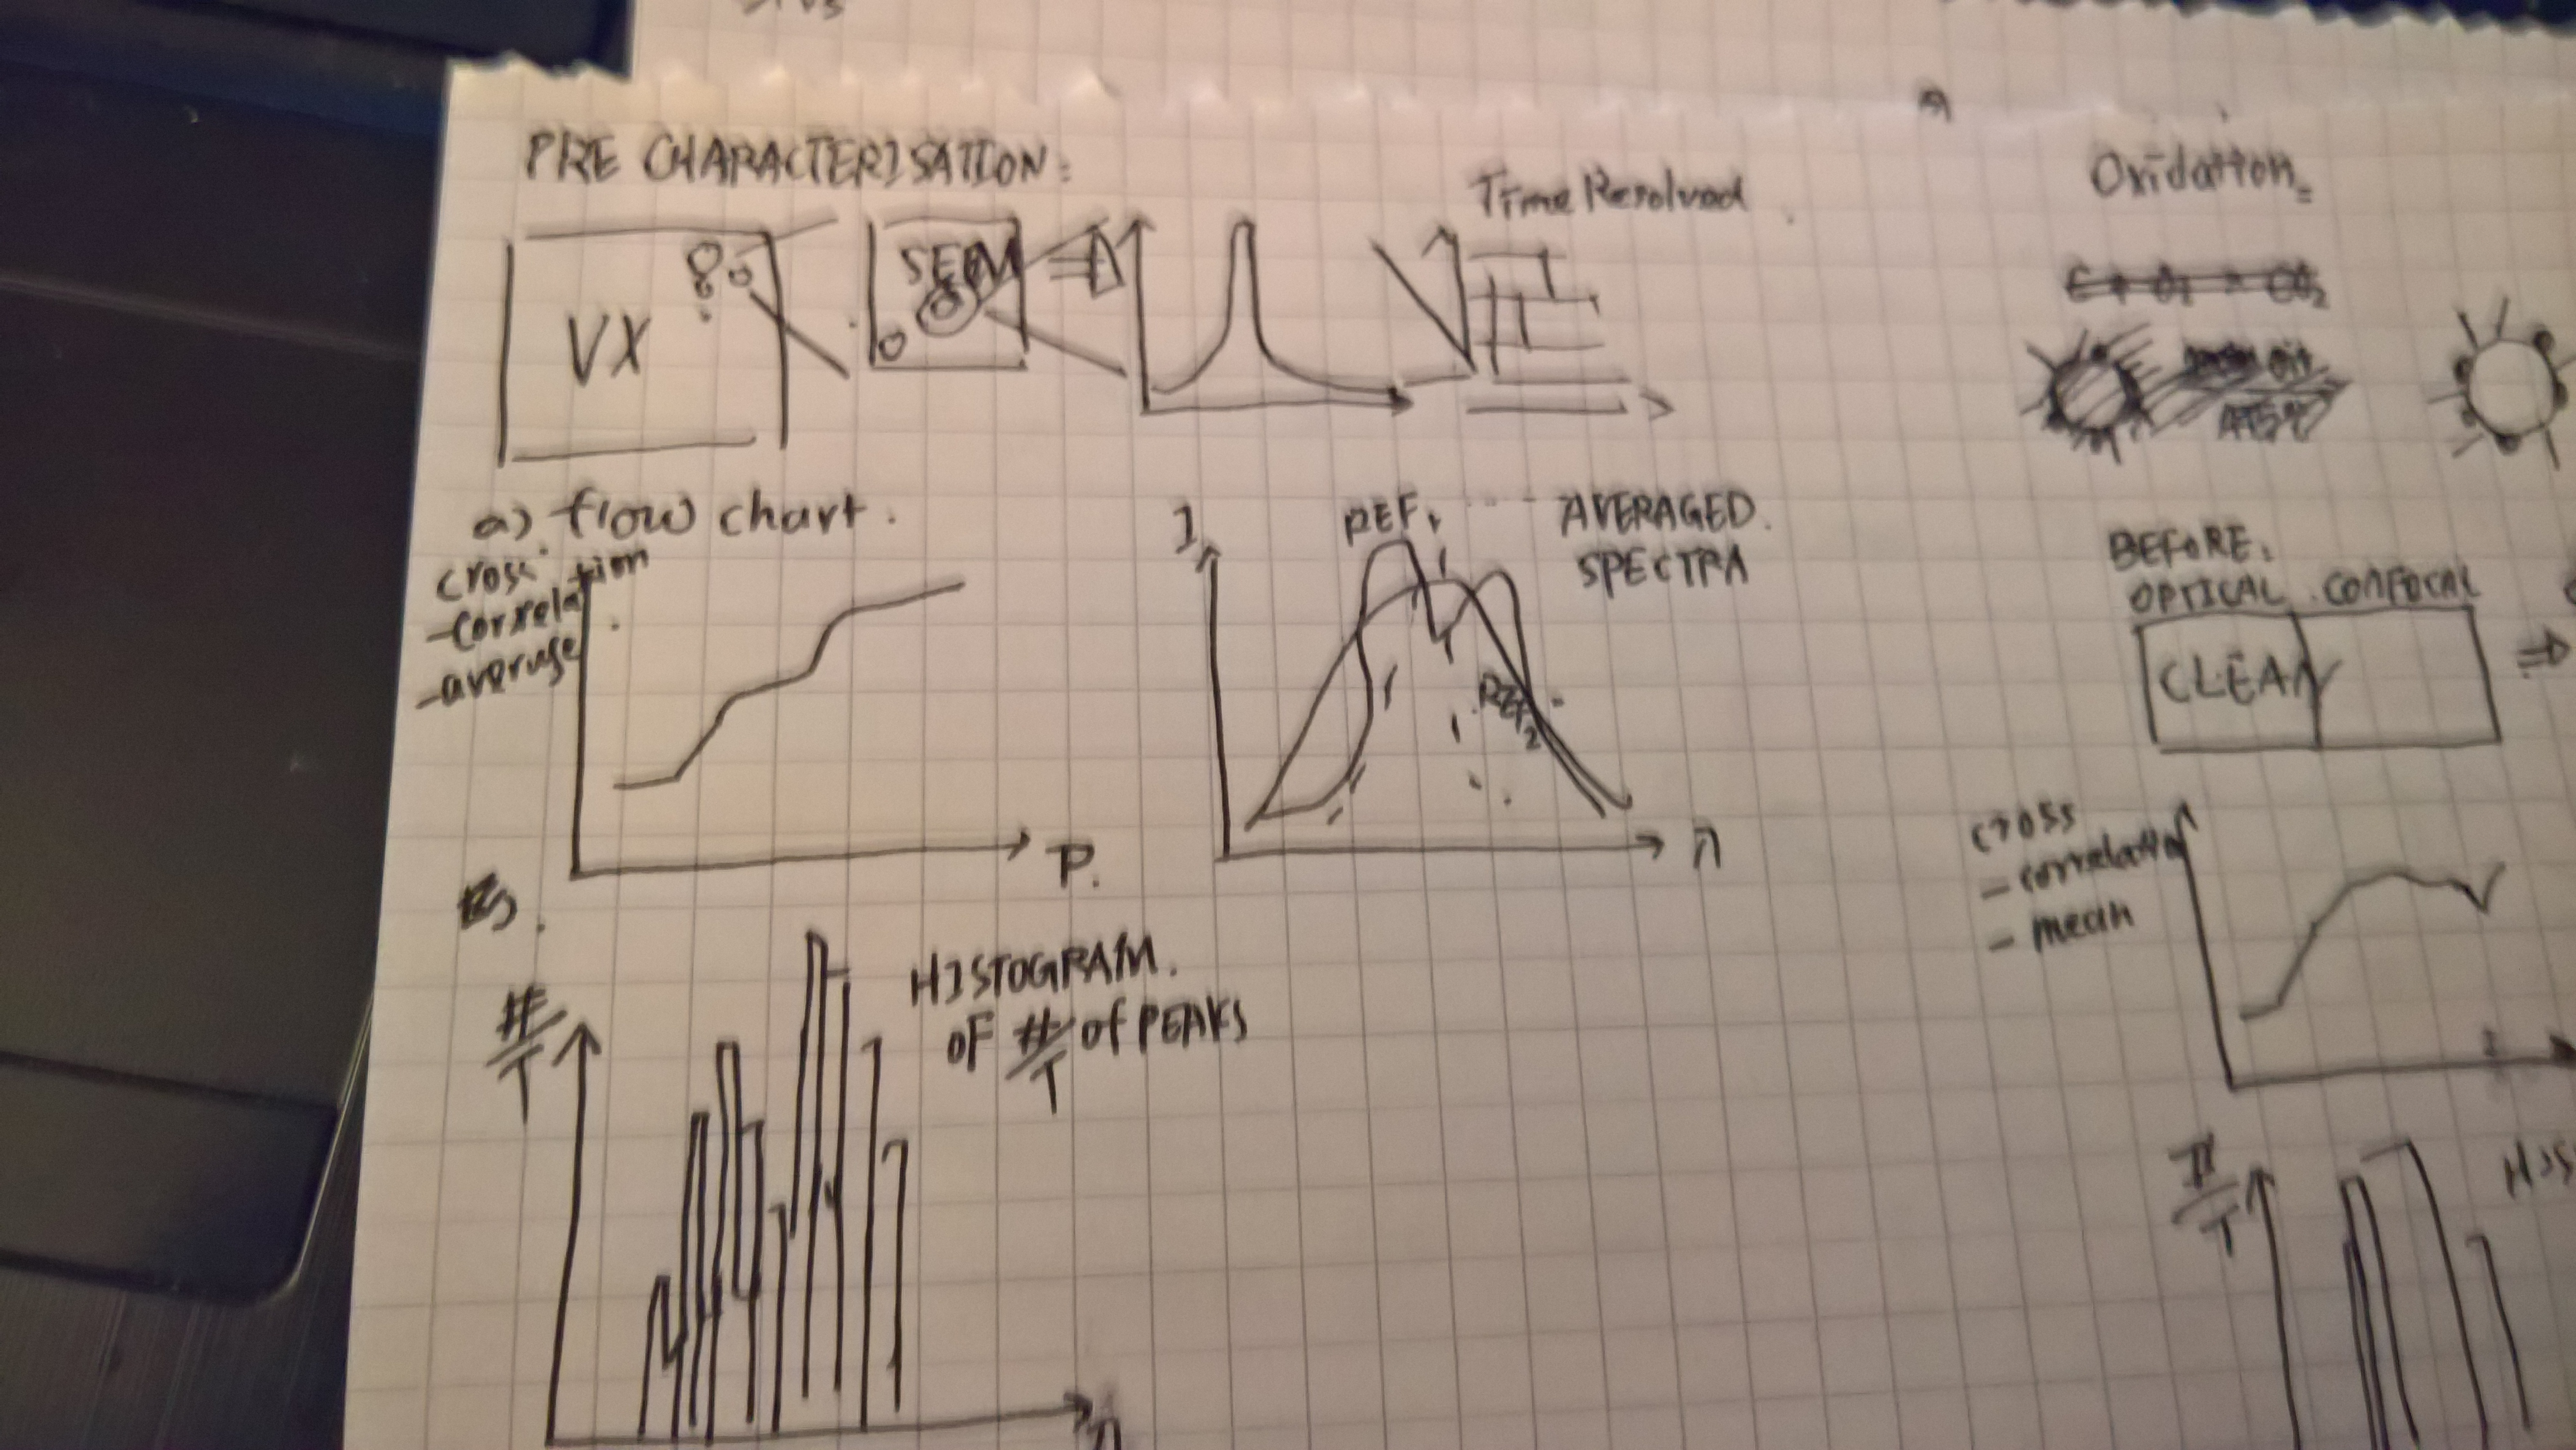
\includegraphics[width=0.7\linewidth]{Figures/pic/WP_20160921_20_41_03_Pro_LI}
\caption{}
\label{fig:wp20160921204103proli}
\end{figure}
\FloatBarrier
\paragraph{post-oxidation characterisation}
1. Optical microscopy check
The first thing we found after the oxidation is that, the surface of our sample turned very dirty. We are yet not certain about what the contaminations are, are they intrinsic or are they external. A possible deduction is that, the contamination comes from the glass tube of tube furnace, that the residues of previous treatments has attached to the inner surface of the tube and evaporized again, depositing on the surface of our sample. Further improvement of oxidation operation has been done in our second oxidation test, and will be mentioned in the next part of the thesis.


2. confocal microscopy imaging and PL spectra.
Huge amount of bright spots can be seen in the confocal image when we excite the sample with 532nm green laser. There's no Silicon vacancy like spectra found in these bright spots. We refind our points of interests next to the marker 4C. The photoluminescence spectra shows much higher intensity than before the oxidation.


3. Cold spectra and PLE 
After the confirmation of points of interests, the sample was transfered into the flow cryostat and the helium flow brought the temperature down to 4.8K.

At 4.8K we recorded the time-resolved photoluminescence spectra of different incident beam power with an excitation wavelength of 532nm. 

After the first oxidation, we learned that due to the inner strain of photonic fibre, the incident beam can not preserve a static polarisation. To stable the polarisation, we used a polarising beam spliter with a LC noise eater behind it. This would fix the polarisation at vertical direction.
\FloatBarrier
\begin{figure}[h]
\centering
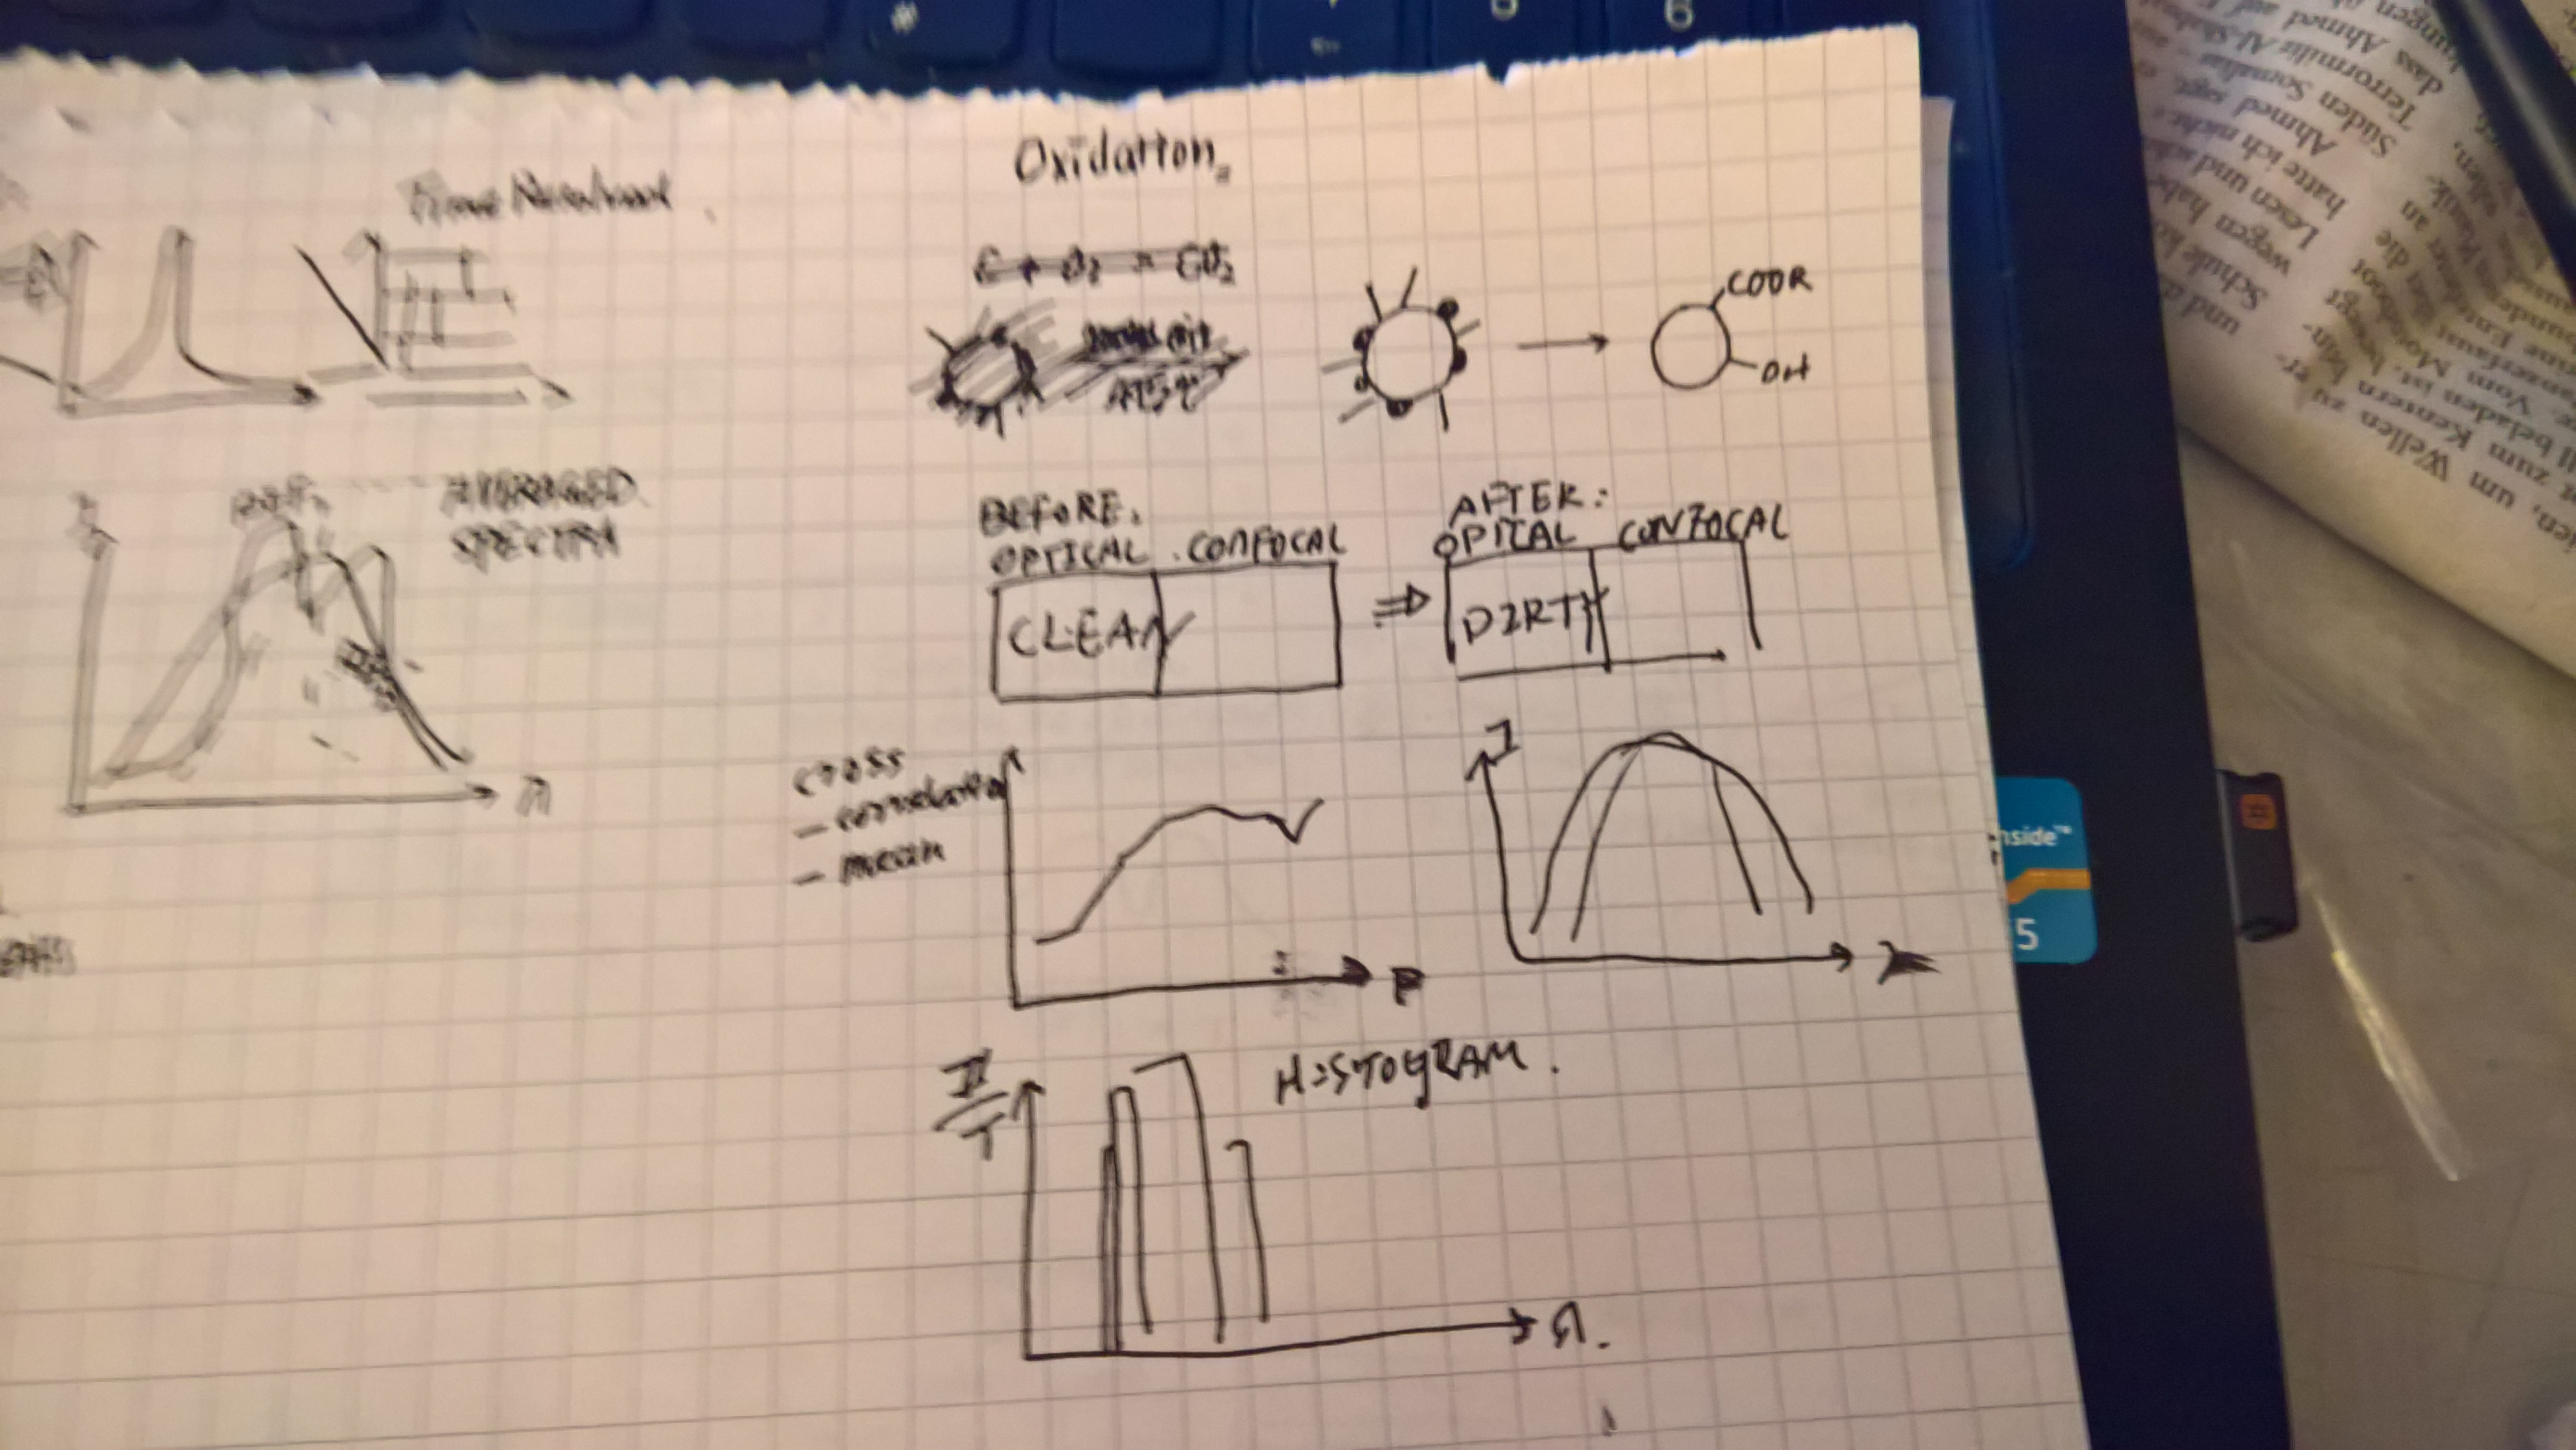
\includegraphics[width=0.7\linewidth]{Figures/pic/WP_20160921_20_41_09_Pro_LI}
\caption{}
\label{fig:wp20160921204109proli}
\end{figure}
\FloatBarrier

\paragraph{Analysis}
After the oxidation we noticed an increased intensity of emission,both background and the 737nm line. The number of lines per spectrum has decreased, while before the oxidation, fine lines ranging from  

\subsection[Second Oxidation]{second Oxidation}

\paragraph{method} As is mentioned before, the optical properties of SiV in bulk diamond is extraordinary. Most importantly, the spectrodiffusion that we have observed in nanodiamonds has never been seen in bulk diamonds. In the first oxidation, it seems the removal of graphitic impurity didn't help with the stablization of emiision lines. In this second oxidation, we decided to used a higher temperature to acquire a surface with groups that imitates the bulk diamond.As reported by [paper], after 2 hours of aerobatic oxidation at $575^{o}C$, ... here insert a sentence of the surface groups of nanodiamonds. To increase the chance of finding smaller nanodiamonds that would fit into a cavity and decrease the chance of getting clusters of nanodiamonds, this time we chose to use nanodiamond of the first batch. These nanodiamond are spin coated on the substrate following the method II(the index, can be change).
\FloatBarrier
\begin{figure}[h]
\centering
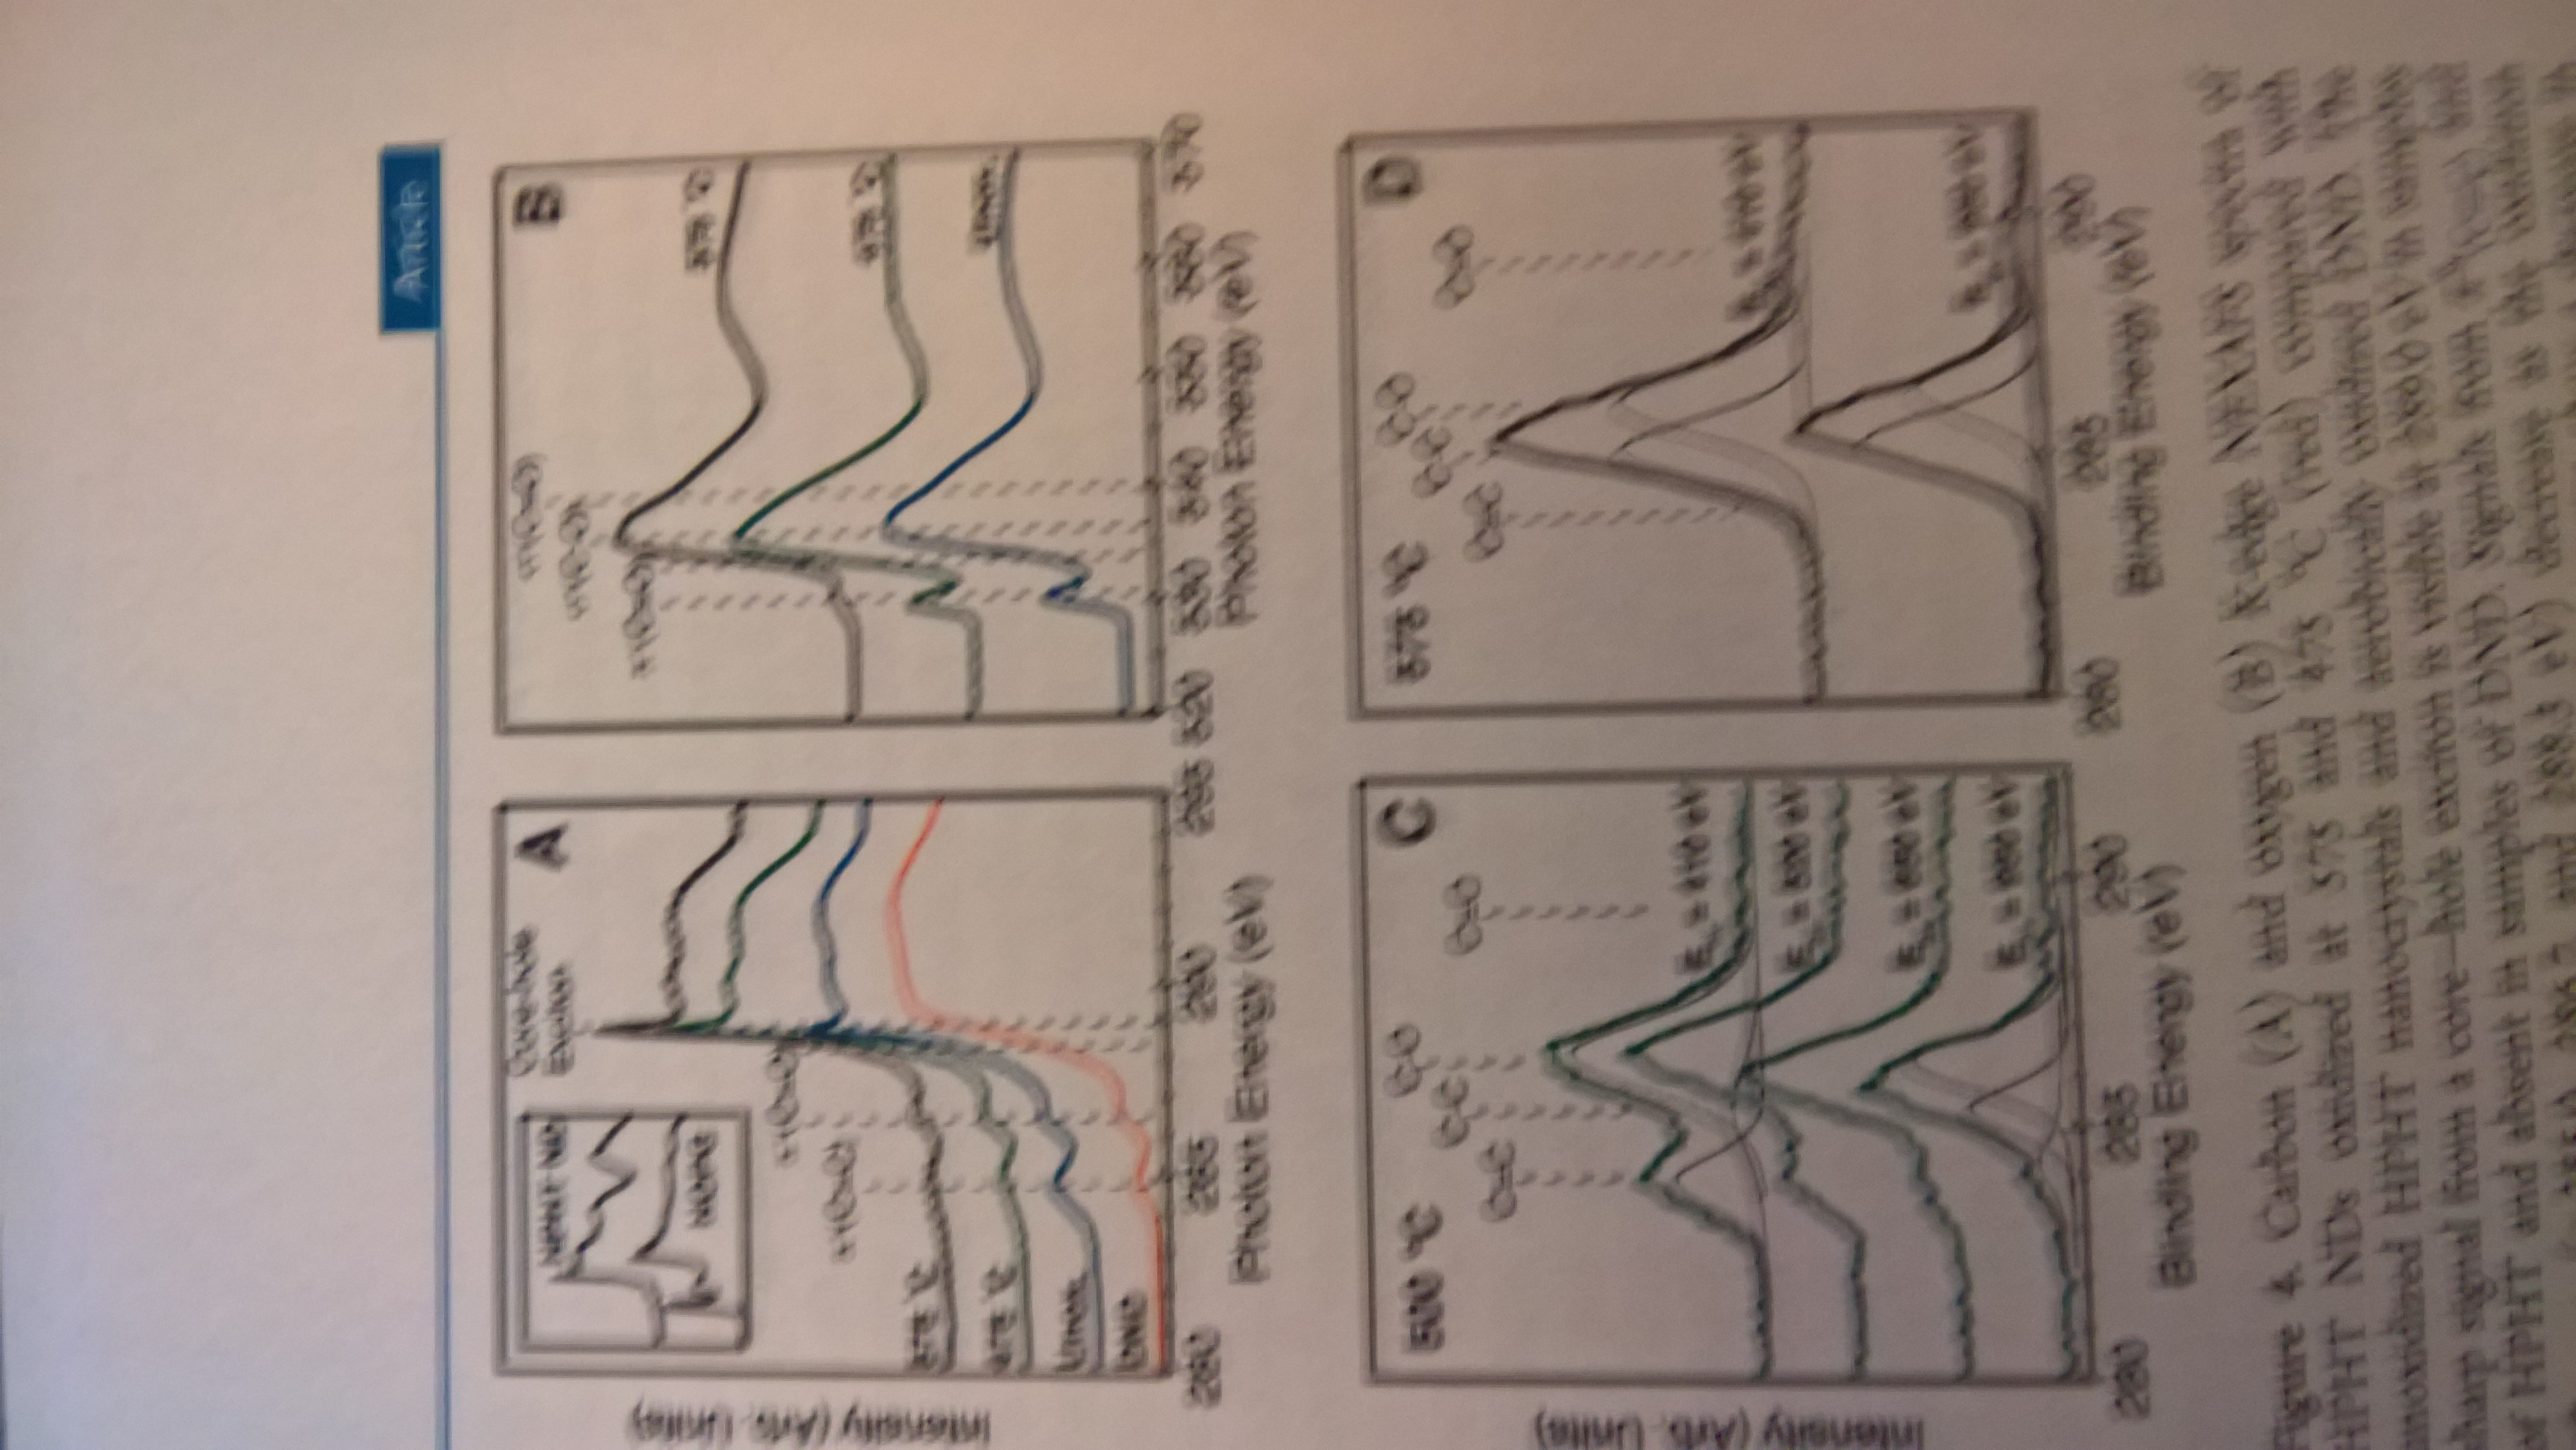
\includegraphics[width=0.7\linewidth]{Figures/pic/WP_20160921_20_42_21_Pro_LI}
\caption{}
\label{fig:wp20160921204221proli}
\end{figure}
\FloatBarrier
Taking the experiences of last oxidation into consideration. This time we introduces flowing inert gas (helium) to flush away the potential contaminations during the cooling process. This can also prevent the result to be affected by the humidity of the air.
We found out the extinction rate of polarising beam spliter is not ideal, so this time we used a Clan Thompson polarisation filter instead.

\paragraph{Before Oxidation}
1.Optical microscopy observation
\FloatBarrier
\begin{figure}[h]
\centering
\includegraphics[width=0.7\linewidth]{Figures/pic/20150907_sample214_spincoated_5}
\caption{}
\label{fig:20150907sample214spincoated5}
\end{figure}
\FloatBarrier  
THIS IS NOT THE RIGHT FIGURE NEED CHECK THE SERVER
We observed the sample after the spin coating with optical microscopy, the surface appeared to be relatively clean, little amount of contamination has been observed, but is acceptable.

2.Mapping of $SiV^{-}$ with room temperature setup.
\FloatBarrier
\begin{figure}[h]
\centering
\includegraphics[width=0.7\linewidth]{Figures/pic/dc}
\caption{}
\label{fig:dc}
\end{figure}
\FloatBarrier
Once again, we exxplored the sample with the same room temperature confocal microscopy setup. With the help of spectrometer, we find a few points of interest with a emission spectrum that resembles $SiV^{-}$. 

3. Cold time-resolved PL and exitation polarisation

As has been mention in last chapter, it is suspect that the incident polarisation can affect the spectral behaviour of SiV. We added in the excitation polarisation measurement and recorded the time resolved photoluminescence spectra of 2 different excitation polarisation that are perpendicular to each other. This is achieved by putting a motor-driven half-lambda plate after the noise eater. 
Due to short time scheme from this measurement we decided to fix the input power at [?need to check], which is the lowest power that can offer most of the points of interest's a decent signal to noise ration.
\FloatBarrier
\begin{figure}[h]
\centering
\includegraphics[width=0.7\linewidth]{Figures/pic/WP_20160921_21_04_59_Moment}
\caption{}
\label{fig:wp20160921210459moment}
\end{figure}
\FloatBarrier



\paragraph{After Oxidation} 

1. Optical Microscopy observation. 

After the Oxidation, we found the surface not as dirty as the last Oxidation. It seems a cleaner tube and flowing gas flushing do have helped suppressing the surface contamination introduced by the tube furnace.
2. Room temperature mapping
\FloatBarrier
\begin{figure}[h]
\centering
\includegraphics[width=0.7\linewidth]{Figures/pic/WP_20160921_21_05_04_Moment}
\caption{}
\label{fig:wp20160921210504moment}
\end{figure}
\FloatBarrier



\paragraph{Analysis} 
Comparasion if possible: different behaviour pre treatment between two batches
Possible reason: losing NDs due to Helium flow while cooling, GR1 getting closer to the surface due to oxidation caused size/thickness reduction.

%----------------------------------------------------------------------------------------
%	SECTION 4
%----------------------------------------------------------------------------------------

\section[H termination]{H termination}
\paragraph{Effect of H termination}

NEA, band structure of diamond. Reduction of surface.
\FloatBarrier
\begin{figure}[h]
\centering
\includegraphics[width=0.7\linewidth]{Figures/pic/WP_20160921_21_05_16_Pro_LI}
\caption{}
\label{fig:wp20160921210516proli}
\end{figure}
\FloatBarrier
\paragraph{method} Plasma treatment, setup, apparatus.
ASK OSCHDI TO SEND THE PARAMETERS

\paragraph{why no pre characterisation} Conditions for Plasma treatment.
Vaccum and clean surface.
\paragraph{After H termination} Confocal image, optical image, excitation polarisation, time resolved PL with different incident polarisation.
\FloatBarrier
\begin{figure}[h]
\centering
\includegraphics[width=0.7\linewidth]{Figures/pic/WP_20160921_21_05_13_Pro_LI}
\caption{}
\label{fig:wp20160921210513proli}
\end{figure}
\FloatBarrier

\paragraph{Analysis} Within the instrumental limit of spectrometer, the spectral diffusion has been significantly suppressed. Possible reason.